%!TEX root = ../../../2019main.tex
\vspace{10pt}
\subsubsection*{\bf Vibration Isolation System Type-A}
\vspace{3pt}
\noindent {\sf [Spokesperson :\ Lucia TROZZO]}

\vspace{3pt}
\noindent {\sf \small ICRR, The Univ.\ of Tokyo, Hida, Gifu 506-1205}
lucia,s contribution
%
\subsubsection*{\bi Introduction}
Seismic noise gives the most important contribution and it is dominant in the range [0.1,10] Hz. This region is critical for the ground based GW detector, because the seismic noise influence the detector sensitivity and the possibility to operate with high duty cycle: The selection of an experimental site has a key role to limit the impact of seismic noise on interferometric detectors for Gravitational Waves observations. In underground locations the perturbations caused by the atmospheric fluctuation due to the weather conditions are minimal, the environmental conditions are more stable and, as a consequence, the measurable noise on the surface level is attenuated: seismic noise, in the underground facilities, is about 100 time smaller than those ones on surface:  for all these reasons  KAGRA has been designed to be underground.
Anyway to achieve the target sensitivity of  $10^{-18}$\, m/sqrt(Hz) at 10 Hz, suspending optical components is a crucial task in the construction of GW interferometers. In fact the gravitational waves observation depends on the capability to include into the experimental apparatus a free falling mass (test mass), well isolated from all the noise sources which are relevant in the observational frequency band.
For these reasons the ground based and broad-band interferometers have been equipped with an appropriate suspension system of the test masses including complex mechanical structures studied to inhibit noise transmission and consider test masses as free-falling from few Hz.


\begin{figure}[hbtp]
\begin{center}
\includegraphics[width=0.48\textwidth]{astrodiv/gw/vis-a/Kagraseismicnoise.jpeg}
\caption{\utsm \noindent{\narrower{Seismic noise spectrum on surface in the Tokyo area and the measurements performed at differents levels inside the Kamioka mine}}}
\label{fig:KAGRAseismicnoise}

\end{center}
\end{figure}

\paragraph*{\bi Vibration Isolation System for the Cryogenic Mirrors: Type A }
A good approximation of a free falling mass is represented by a simple pendulum composed by a thin wire, as elastic element, connected to a body of mass m . Thanks to this simple solution it is possible to filter seismic noise in a real experiment to the optical level by using a harmonic oscillator. In GW detectors seismic isolation with a capability attenuation ~ 10 orders of magnitude is needed: It is evident that a multiple stage pendulum represents a good approach to improve the total attenuation factor of seismic noise at the level of the test masses. Solution adopted in KAGRA is based on the idea to replicate harmonic oscillators of length ~ 2 m to obtain a sophisticated mechanical structure: Type-A suspensions.
The Type-A suspension is a nine-stage pendulum with the height of 13.5 m based on the second floor of the underground mine. The top of the suspension has a pre-isolation stage supported by three inverted pendulum legs. The suspension chain consists of cascaded geometric anti-spring filters that show low frequency mechanical resonances. 
The bottom four stages including the sapphire mirror are called cryogenic payload and cooled down to about 20\, K in order to reduce the thermal noises. The whole suspension provide a seismic attenuation of ~ $15$\, orders of magnitude at 10 Hz.

\begin{figure}[hbtp]
\begin{center}
\includegraphics[width=0.48\textwidth]{astrodiv/gw/vis-a/TypeAoverwiew.jpeg}
\caption{\utsm \noindent{\narrower{Drawing of the Type A suspension system }}}
\label{fig:TytpeA}

\end{center}
\end{figure}
The suspension system has a negative aspect of amplifying the mirror fluctuation at its resonant frequencies: the excess of the mirror displacement even at an out-of-band frequency disturbs stable operation of the interferometer. We need to implement damping controls on suspension stage and on the payload, in order reduce the free swinging of the test masses and to make the system robust against external disturbances. 
\begin{figure}[hbtp]
\begin{center}
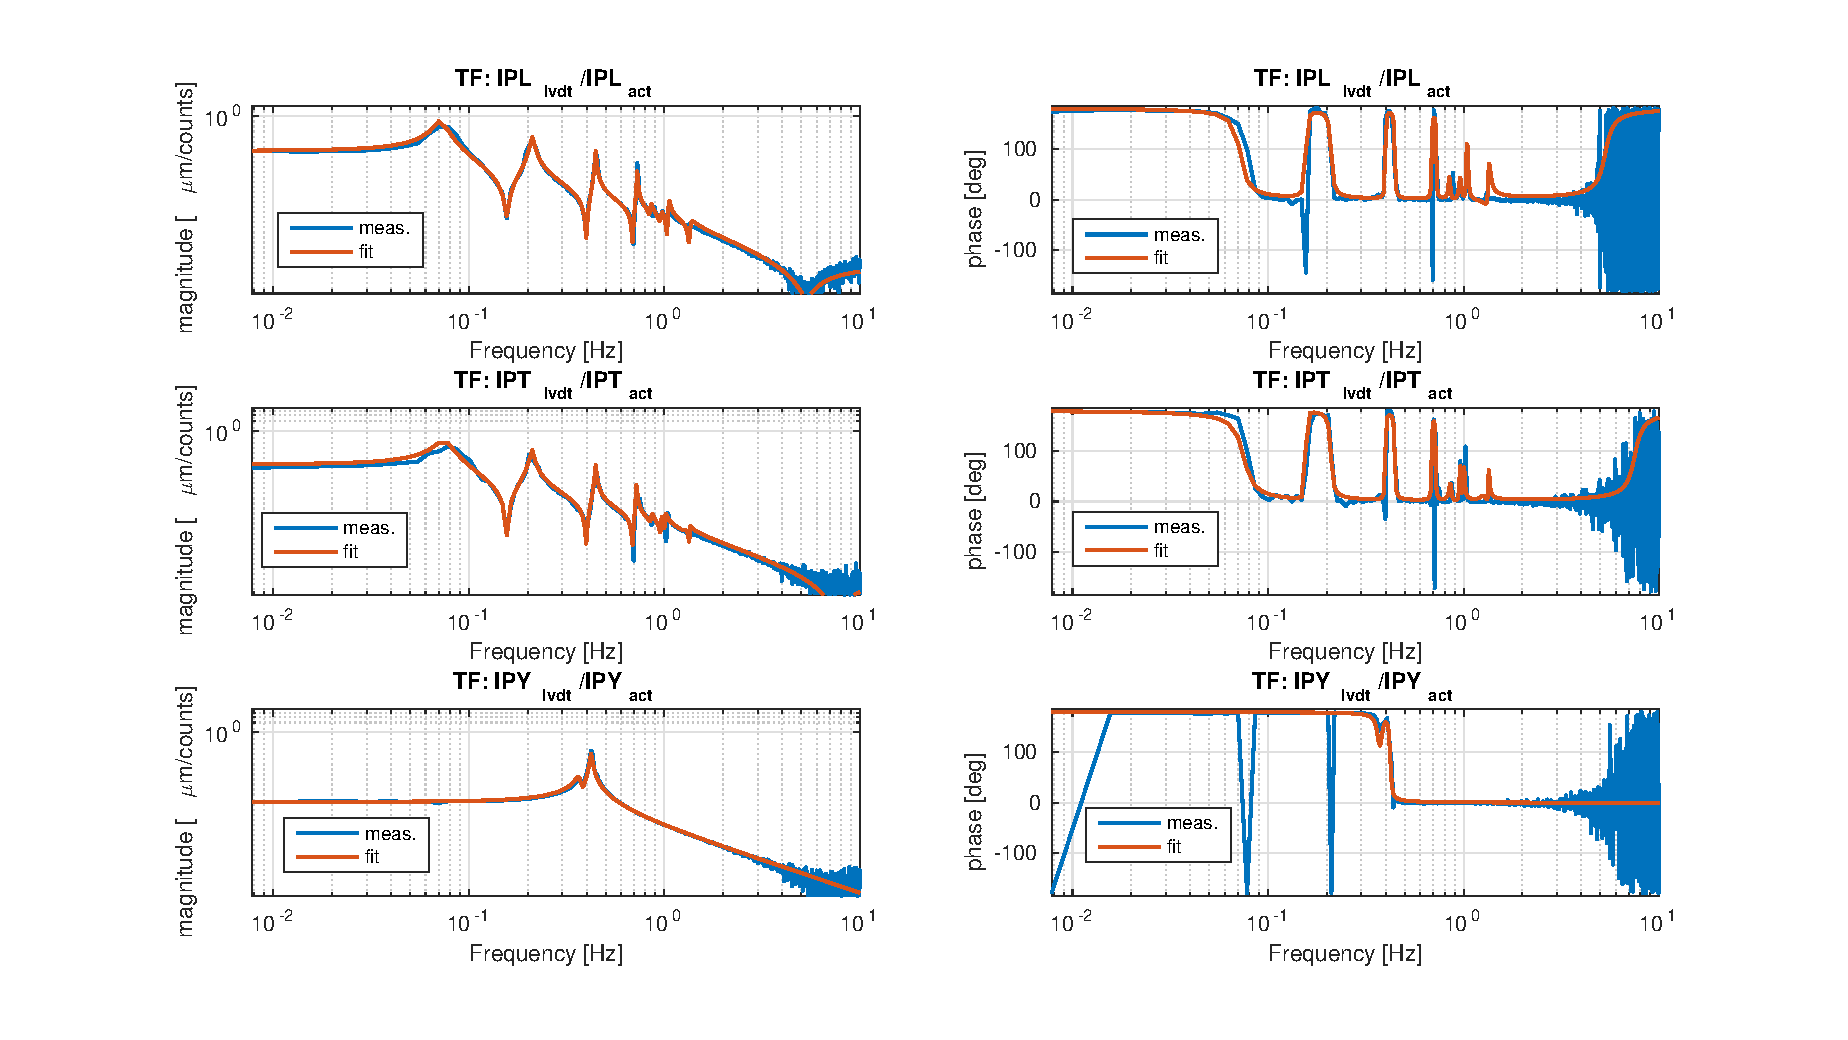
\includegraphics[width=0.48\textwidth]{astrodiv/gw/vis-a/TypeATF.eps}
\caption{\utsm \noindent{\narrower{Normal modes of Type A suspension system }}}
\label{fig:TytpeATF}

\end{center}
\end{figure}

To monitor and control the displacement of the suspension, the system is equipped with several sensors and actuators: position sensors (LVDT), inertial sensors (accelerometer or geophone), photosensors, optical levers, actuators (coil-magnet type). Thanks to the presence of these sensors and actuators a feedback control could be implemented in different points: Inverted Pendulum, vertical GAS filters, Bottom Filter, Marionette stage and the Mirror.
The intent of the feedback action is to reduce the swinging of the free falling masses along:
-longitudinal, transverse direction by acting on the Top stage (IP);
- vertical direction by acting on GAS filters;
- angular directions (Pitch and Yaw) by acting on the Bottom Filter, the Marionette and the Intermediate mass stages.
At the IP stage the "sensor correction technique" and the "tidal compensation" are also implemented. Thanks to them it is possible to achieve a suppression of microseismic noise, in the range [0.1 0.5] Hz, by about a factor 3 and to compensate for long-term drifts in Fabry-Perot cavities due to the tidal effect, respectively.
All these control loops play a crucial role in the locking acquisition process of the whole interferometer: in fact they are engaged to achieve and to keep its standard working conditions even after a violent unlock event.













